  \section{Finite Volume Method for Incompressible Flows -- Theoretical Basics}

  This section deals with the fundamentals of the numerical solution via a finite volume method of the formerly presented set of partial differential equations. The focus of this section is, to provide an overview over the methods to be used in the present thesis. The information contained in this section is based on (Peric,Schäfer,Muzaferja,Jsak). The overview starts by mentioning the different grid types to be used and the discretization techniques to be applied. On the basis of integral formulations of the equations to be solved, the therein contained integrals and differential operators have to be discretized. Since the accuracy of the default concepts for discretizing differential operators degrades with decreasing grid quality, this chapter furthermore presents different approaches to handle corrections for cases in which the cause of degrading grid quality is increased non-orthogonality. 
  
 The goal of the finite volume method is to provide algebraic equations which can be used to determine an approximate solution of a partial differential equation. This system of linear algebraic equations can be solved by means of algorithms to be presented in the end of this section. However since the Navier-Stokes equations are in general non-linear an intermediate step has to be taken, by linearizing the discrete equations. This leads to the need of an iteration process, the \textit{Picard iteration}, which will be explained briefly.
      
  \subsection{Numerical Grid}

  In this subsection a brief overview of the general grid structure to be used in the present thesis is given. The main idea behind finite volume methods is to solve partial differential equations by integrating them over the specified continuous problem domain and dividing this domain into a finite number of subdomains, the so called control volumes. The result of the this finite partition of a continuous problem domain is called the numerical grid. The grid consists of a finite number of grid cells which represent the boundaries of a discrete domain of integration. Depending on whether the numerical solution of an equation is to be calculated on the boundary vertices of grid cell or in the center of the cell, the variable arrangement is denoted to be vertex or cell center oriented. As the methods of employed in the present thesis are intended to be generally applicable to complex geometries the cell centered approach offers more flexibility (\ref{fig:cellvertex}). DONT CONFUSE WITH STAGGERED AND COLLOCATED ARRANGEMENT.

  \begin{figure}
     \label{fig:cellvertex}
      \subfigure{
      \begin{minipage}[1\width]{0.5\textwidth}%
        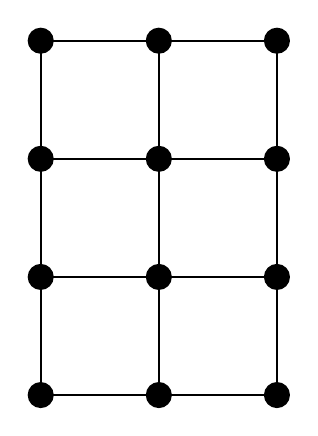
\begin{tikzpicture}

  \draw[thick] (0,0) rectangle (3,4.5);
  \draw[step=15mm,thick] (0,0) grid (3,4.5);

  \node at (0.0,0.0) [circle,fill=black] {};
  \node at (1.5,0.0) [circle,fill=black] {};
  \node at (3.0,0.0) [circle,fill=black] {};

  \node at (0.0  ,1.5) [circle,fill=black] {};
  \node at (1.5,1.5) [circle,fill=black] {};
  \node at (3.0,1.5) [circle,fill=black] {};

  \node at (0.0,3) [circle,fill=black] {};
  \node at (1.5,3) [circle,fill=black] {};
  \node at (3.0,3) [circle,fill=black] {};

  \node at (0.0,4.5) [circle,fill=black] {};
  \node at (1.5,4.5) [circle,fill=black] {};
  \node at (3.0,4.5) [circle,fill=black] {};


\end{tikzpicture}

        \centering{}
      \end{minipage}}\qquad
      \subfigure{
      \begin{minipage}[1\width]{0.4\textwidth}%
        \centering{}
        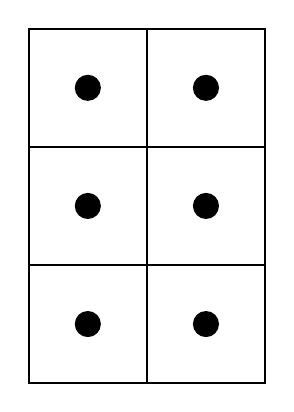
\begin{tikzpicture}

  \draw[thick] (0,0) rectangle (3,4.5);
  \draw[step=15mm,thick] (0,0) grid (3,4.5);

  \node at (0.75,0.75) [circle,fill=black] {};
  \node at (0.75,2.25) [circle,fill=black] {};
  \node at (0.75,3.75) [circle,fill=black] {};

  \node at (2.25,0.75) [circle,fill=black] {};
  \node at (2.25,2.25) [circle,fill=black] {};
  \node at (2.25,3.75) [circle,fill=black] {};

\end{tikzpicture}

      \end{minipage}}
      \caption{Comparison of vertex oriented and cell center oriented variable arrangement}
  \end{figure}

    Regarding the treatment of domain boundaries and the ordering of the cells within the problem domain different types of numerical grids can be distinguished. The present thesis makes use of so called block structured grids with hexahedron cells. A structured grid is characterized by a constant amount of of grid cells in each coordinate direction. The high regularity of structured grids benefits the computational efficiency of algorithms to be used on this type of grid. A block structured grid consists of different grid blocks of which each considered individually is structured, but if the topology of the grid is considered it is unstructured. An example of a block structured grid with distinguishable grid blocks is given in figure \ref{fig:blockstruc}. The use of block structured grids is motivated by the need to increase the adaptivity of structured grids by maintaining high computational efficiency. Furthermore it naturally embraces the concept of domain decomposition which facilitates the implementation of parallel algorithms for the decomposed computational domain.

    Inside a structured grid block, cells with the shape of hexahedrons are used. In addition to the geometric boundaries of each control volume a numerical grid also provides a mapping that assigns to each control volume with index \(P\) a set of indexes of neighbouring control volumes \(NB(P):=\{W,S,B,T,N,E\}\), which are named after the geographic directions. Figure \ref{fig:blockstruc} shows a single grid cell with its direct neighbours. The faces \(\{S_w,S_s,S,b,S_t,S_n,S_e\}\) of each hexahedral control volume represent the mentioned geometric boundaries. 

    \begin{itemize}
      \item talk about grid quality
      \item talk about local refinement
      \item talk about variable arrangement
    \end{itemize}

    \begin{figure}[h]
      \label{fig:blockstruc}
      \subfigure{
      \begin{minipage}[1\width]{0.5\textwidth}%
        \begin{tikzpicture}
	\coordinate (P1) at (-25cm,6.5cm); % left vanishing point (To pick)
	\coordinate (P2) at (18cm,5.5cm); % right vanishing point (To pick)

	\coordinate (A1) at (0em,0cm); % central top point (To pick)
	\coordinate (A2) at (0em,1.5cm); % central bottom point (To pick)
	\coordinate (A3) at (0em,3cm); % central bottom point (To pick)

	\coordinate (A4) at ($(P1)!.94!(A1)$); 
	\coordinate (A5) at ($(P1)!.94!(A2)$);
	\coordinate (A6) at ($(P1)!.94!(A3)$);

	\coordinate (A7) at ($(P1)!.88!(A1)$); 
	\coordinate (A8) at ($(P1)!.88!(A2)$);
	\coordinate (A9) at ($(P1)!.88!(A3)$);

	\coordinate (A10) at ($(P2)!.94!(A1)$); 
	\coordinate (A11) at ($(P2)!.94!(A2)$);
	\coordinate (A12) at ($(P2)!.94!(A3)$);

	\coordinate (A19) at ($(P2)!.88!(A1)$); 
	\coordinate (A20) at ($(P2)!.88!(A2)$);
	\coordinate (A21) at ($(P2)!.88!(A3)$);

	\coordinate (A13) at
	  (intersection cs: first line={(A10) -- (P1)},
			    second line={(A4) -- (P2)});
	\coordinate (A14) at
	  (intersection cs: first line={(A11) -- (P1)}, 
			    second line={(A5) -- (P2)});
	\coordinate (A15) at
	  (intersection cs: first line={(A12) -- (P1)}, 
			    second line={(A6) -- (P2)});

	\coordinate (A16) at
	  (intersection cs: first line={(A10) -- (P1)},
			    second line={(A7) -- (P2)});
	\coordinate (A17) at
	  (intersection cs: first line={(A11) -- (P1)}, 
			    second line={(A8) -- (P2)});
	\coordinate (A18) at
	  (intersection cs: first line={(A12) -- (P1)}, 
			    second line={(A9) -- (P2)});

	\coordinate (A22) at
	  (intersection cs: first line={(A19) -- (P1)},
			    second line={(A4) -- (P2)});
	\coordinate (A23) at
	  (intersection cs: first line={(A20) -- (P1)}, 
			    second line={(A5) -- (P2)});
	\coordinate (A24) at
	  (intersection cs: first line={(A21) -- (P1)}, 
			    second line={(A6) -- (P2)});

	\coordinate (A25) at
	  (intersection cs: first line={(A19) -- (P1)},
			    second line={(A7) -- (P2)});
	\coordinate (A26) at
	  (intersection cs: first line={(A20) -- (P1)}, 
			    second line={(A8) -- (P2)});
	\coordinate (A27) at
	  (intersection cs: first line={(A21) -- (P1)}, 
			    second line={(A9) -- (P2)});

        \foreach \i in {1,2,3,4,5,6,7,8,9,
                        10,11,12,15,18,
                        19,20,21,24,27}
        {
	 %\draw[fill=black] (A\i) circle (0.15em) ;
        }

        %Vertical Lines
        \draw (A1) -- (A2) -- (A3);
        \draw (A4) -- (A5) -- (A6) -- (A15) -- (A24);
        \draw (A7) -- (A8) -- (A9) -- (A18) -- (A27);
        \draw (A12) -- (A15) -- (A18);
        \draw (A21) -- (A24) -- (A27);

        \fill[gray!30] (A1) -- (A19) -- (A21) -- (A3) -- cycle;
        %Horizontal Lines
        \draw (A7) -- (A4) -- (A1);
        \draw (A8) -- (A5) -- (A2);
        \draw (A9) -- (A6) -- (A3) -- (A12) -- (A21);
        \draw[gray,dashed] (A2) -- (A20);
        \draw[gray,dashed] (A10) -- (A12);
        \draw[gray,dashed] (A1) -- (A19);
        \draw[gray,dashed] (A19) -- (A21);

        %Boundary

	\coordinate (B1) at (0em,0cm);
	\coordinate (B2) at (0em,1cm);
	\coordinate (B3) at (0em,2cm);
	\coordinate (B4) at (0em,3cm);

	\coordinate (B5) at ($(P1)!1.05!(B1)$); 
	\coordinate (B6) at ($(P1)!1.05!(B2)$);
	\coordinate (B7) at ($(P1)!1.05!(B3)$);
	\coordinate (B8) at ($(P1)!1.05!(B4)$);

	\coordinate (B9)  at ($(P1)!1.1!(B1)$); 
	\coordinate (B10) at ($(P1)!1.1!(B2)$);
	\coordinate (B11) at ($(P1)!1.1!(B3)$);
	\coordinate (B12) at ($(P1)!1.1!(B4)$);

	\coordinate (B13)  at ($(P1)!1.15!(B1)$); 
	\coordinate (B14) at ($(P1)!1.15!(B2)$);
	\coordinate (B15) at ($(P1)!1.15!(B3)$);
	\coordinate (B16) at ($(P1)!1.15!(B4)$);

	\coordinate (B17) at ($(P2)!0.96!(B1)$); 
	\coordinate (B18) at ($(P2)!0.96!(B2)$);
	\coordinate (B19) at ($(P2)!0.96!(B3)$);
	\coordinate (B20) at ($(P2)!0.96!(B4)$);

        \coordinate (B33) at ($(P2)!.92!(B1)$); 
        \coordinate (B34) at ($(P2)!.92!(B2)$);
        \coordinate (B35) at ($(P2)!.92!(B3)$);
        \coordinate (B36) at ($(P2)!.92!(B4)$);

        \coordinate (B49) at ($(P2)!.88!(B1)$); 
        \coordinate (B50) at ($(P2)!.88!(B2)$);
        \coordinate (B51) at ($(P2)!.88!(B3)$);
        \coordinate (B52) at ($(P2)!.88!(B4)$);

	\coordinate (B21) at
	  (intersection cs: first line={(B17) -- (P1)},
			    second line={(B5) -- (P2)});
	\coordinate (B22) at
	  (intersection cs: first line={(B18) -- (P1)},
			    second line={(B6) -- (P2)});
	\coordinate (B23) at
	  (intersection cs: first line={(B19) -- (P1)},
			    second line={(B7) -- (P2)});
	\coordinate (B24) at
	  (intersection cs: first line={(B20) -- (P1)},
			    second line={(B8) -- (P2)});

	\coordinate (B25) at
	  (intersection cs: first line={(B17) -- (P1)},
			    second line={(B9) -- (P2)});
	\coordinate (B26) at
	  (intersection cs: first line={(B18) -- (P1)},
			    second line={(B10) -- (P2)});
	\coordinate (B27) at
	  (intersection cs: first line={(B19) -- (P1)},
			    second line={(B11) -- (P2)});
	\coordinate (B28) at
	  (intersection cs: first line={(B20) -- (P1)},
			    second line={(B12) -- (P2)});

	\coordinate (B29) at
	  (intersection cs: first line={(B17) -- (P1)},
			    second line={(B13) -- (P2)});
	\coordinate (B30) at
	  (intersection cs: first line={(B18) -- (P1)},
			    second line={(B14) -- (P2)});
	\coordinate (B31) at
	  (intersection cs: first line={(B19) -- (P1)},
			    second line={(B15) -- (P2)});
	\coordinate (B32) at
	  (intersection cs: first line={(B20) -- (P1)},
			    second line={(B16) -- (P2)});

	\coordinate (B37) at
	  (intersection cs: first line={(B33) -- (P1)},
			    second line={(B5) -- (P2)});
	\coordinate (B38) at
	  (intersection cs: first line={(B34) -- (P1)},
			    second line={(B6) -- (P2)});
	\coordinate (B39) at
	  (intersection cs: first line={(B35) -- (P1)},
			    second line={(B7) -- (P2)});
	\coordinate (B40) at
	  (intersection cs: first line={(B36) -- (P1)},
			    second line={(B8) -- (P2)});

	\coordinate (B41) at
	  (intersection cs: first line={(B33) -- (P1)},
			    second line={(B9) -- (P2)});
	\coordinate (B42) at
	  (intersection cs: first line={(B34) -- (P1)},
			    second line={(B10) -- (P2)});
	\coordinate (B43) at
	  (intersection cs: first line={(B35) -- (P1)},
			    second line={(B11) -- (P2)});
	\coordinate (B44) at
	  (intersection cs: first line={(B36) -- (P1)},
			    second line={(B12) -- (P2)});

	\coordinate (B45) at
	  (intersection cs: first line={(B33) -- (P1)},
			    second line={(B13) -- (P2)});
	\coordinate (B46) at
	  (intersection cs: first line={(B34) -- (P1)},
			    second line={(B14) -- (P2)});
	\coordinate (B47) at
	  (intersection cs: first line={(B35) -- (P1)},
			    second line={(B15) -- (P2)});
	\coordinate (B48) at
	  (intersection cs: first line={(B36) -- (P1)},
			    second line={(B16) -- (P2)});

	\coordinate (B53) at
	  (intersection cs: first line={(B49) -- (P1)},
			    second line={(B5) -- (P2)});
	\coordinate (B54) at
	  (intersection cs: first line={(B50) -- (P1)},
			    second line={(B6) -- (P2)});
	\coordinate (B55) at
	  (intersection cs: first line={(B51) -- (P1)},
			    second line={(B7) -- (P2)});
	\coordinate (B56) at
	  (intersection cs: first line={(B52) -- (P1)},
			    second line={(B8) -- (P2)});

	\coordinate (B57) at
	  (intersection cs: first line={(B49) -- (P1)},
			    second line={(B9) -- (P2)});
	\coordinate (B58) at
	  (intersection cs: first line={(B50) -- (P1)},
			    second line={(B10) -- (P2)});
	\coordinate (B59) at
	  (intersection cs: first line={(B51) -- (P1)},
			    second line={(B11) -- (P2)});
	\coordinate (B60) at
	  (intersection cs: first line={(B52) -- (P1)},
			    second line={(B12) -- (P2)});

	\coordinate (B61) at
	  (intersection cs: first line={(B49) -- (P1)},
			    second line={(B13) -- (P2)});
	\coordinate (B62) at
	  (intersection cs: first line={(B50) -- (P1)},
			    second line={(B14) -- (P2)});
	\coordinate (B63) at
	  (intersection cs: first line={(B51) -- (P1)},
			    second line={(B15) -- (P2)});
	\coordinate (B64) at
	  (intersection cs: first line={(B52) -- (P1)},
			    second line={(B16) -- (P2)});


        %Front lines
        \draw (B13) -- (B29) -- (B45) -- (B61);
        \draw (B1) -- (B5) -- (B9) -- (B13);
        \draw (B2) -- (B6) -- (B10) -- (B14);
        \draw (B3) -- (B7);
        \draw (B14) -- (B62);

        %Vertical lines
        \draw (B5) -- (B6) -- (B7) -- (B8);
        \draw (B29) -- (B30);
        \draw (B45) -- (B46) -- (B47) -- (B48);
        \draw (B61) -- (B62) -- (B63) -- (B64);
        \draw (B13) -- (B14);
        \draw (B9) -- (B10);
        \draw (B38) -- (B40);
        \draw (B22) -- (B24);
        \draw (B42) -- (B44);

        %horizontal lines
        \draw (B22) -- (B26) -- (B30);

        %linien in die tiefe
        \draw (B6) -- (B22); 
        \draw (B7) -- (B39);
        \draw (B10) -- (B42);
        \draw (B47) -- (B63);
        \draw (B48) -- (B64);
        \draw (B44) -- (B60);

        \draw (B8) -- (B24) -- (B40) -- (B56);

        %Top lines (to east)
        \draw (B4) -- (B8);
        \draw (B20) -- (B24);
        \draw (B36) -- (B40) -- (B44) -- (B48);
        \draw (B52) -- (B56) -- (B60) -- (B64);
        \draw (B38) -- (B46);
        \draw (B39) -- (B47);

        %fill out one CV
        \fill[gray!30] (B42) -- (B43) -- (B39) -- (B38) -- cycle;  %back
        \fill[gray!50] (B22) -- (B38) -- (B39) -- (B23) -- cycle;  %left
        \fill[gray!50,opacity=0.2] (B26) -- (B27) -- (B23) -- (B22) -- cycle;  %front
%       \fill[gray!50,opacity=0.7] (B26) -- (B42) -- (B43) -- (B27) -- cycle;  %right
        \fill[gray!90] (B22) -- (B26) -- (B42) -- (B38) -- cycle;  %bottom
        \fill[gray!90,opacity=0.2] (B23) -- (B27) -- (B43) -- (B39) -- cycle;  %top

        \draw[gray!90,dashed] (B8) -- (B16) -- (B48);
        \draw[gray!90,dashed] (B16) -- (B14);
        \draw[gray!90,dashed] (B32) -- (B30);
        \draw[gray!90,dashed] (B12) -- (B10);
        \draw[gray!90,dashed] (B32) -- (B30);
        \draw[gray!90,dashed] (B7) -- (B15) -- (B47);
        \draw[gray!90,dashed] (B23) -- (B31);
        \draw[gray!90,dashed] (B12) -- (B44);
        \draw[gray!90,dashed] (B26) -- (B28);
        \draw[gray!90,dashed] (B24) -- (B32);
        \draw[gray!90,dashed] (B11) -- (B43);

        \draw[gray!90,dashed] (B17) -- (B20);
        \draw[gray!90,dashed] (B33) -- (B36);
        \draw[gray!90,dashed] (B2) -- (B50);
        \draw[gray!90,dashed] (B3) -- (B51);
        \draw[gray!30,dashed] (B49) -- (B61);

        %right lines (vertical)




        \foreach \i in {1,2,3,4,5,6,7,8,9,10,11,12,13,14,15,16,17,18,19,20,21,22,23,24,25,26,27,28,29,30,31,32,33,34,35,36,37,38,39,40,41,42,43,44,45,46,47,48,49,50,51,52,53,54,55,56,57,58,59,60,61,62,63,64}
        {
	 %\draw[fill=black] (B\i) circle (0.15em) ;
        }
        

\end{tikzpicture}

        \centering{}
      \end{minipage}}\qquad
      \subfigure{
      \begin{minipage}[1\width]{0.4\textwidth}%
        \centering{}
            \begin{tikzpicture}
	%%% Edit the following coordinate to change the shape of your
	%%% cuboid
      
	%% Vanishing points for perspective handling
	\coordinate (P1) at (-25cm,6.5cm); % left vanishing point (To pick)
	\coordinate (P2) at (18cm,5.5cm); % right vanishing point (To pick)

	%% (A1) and (A2) defines the 2 central points of the cuboid
	\coordinate (A1) at (0em,2.0cm); % central top point (To pick)
	\coordinate (A2) at (0em,0.0cm); % central bottom point (To pick)

	%% (A3) to (A8) are computed given a unique parameter (or 2) .8
	% You can vary .8 from 0 to 1 to change perspective on left side
	\coordinate (A3) at ($(P1)!.9!(A2)$); % To pick for perspective 
	\coordinate (A4) at ($(P1)!.9!(A1)$);

	% You can vary .8 from 0 to 1 to change perspective on right side
	\coordinate (A7) at ($(P2)!.92!(A2)$);
	\coordinate (A8) at ($(P2)!.92!(A1)$);

	%% Automatically compute the last 2 points with intersections
	\coordinate (A5) at
	  (intersection cs: first line={(A8) -- (P1)},
			    second line={(A4) -- (P2)});
	\coordinate (A6) at
	  (intersection cs: first line={(A7) -- (P1)}, 
			    second line={(A3) -- (P2)});

	%%% Depending of what you want to display, you can comment/edit
	%%% the following lines

	%% Possibly draw back faces

	\fill[gray!90] (A2) -- (A3) -- (A6) -- (A7) -- cycle; % face 6
        \node (C6) at (barycentric cs:A2=1,A3=1,A6=1,A7=1) { $S_b$};
	
	\fill[gray!50] (A3) -- (A4) -- (A5) -- (A6) -- cycle; % face 3
        \node (C3) at (barycentric cs:A3=1,A4=1,A5=1,A6=1) { $S_w$};
	
	\fill[gray!30] (A5) -- (A6) -- (A7) -- (A8) -- cycle; % face 4
        \node (C4) at (barycentric cs:A5=1,A6=1,A7=1,A8=1) { $S_n$};
	
	\draw[thick,dashed] (A5) -- (A6);
	\draw[thick,dashed] (A3) -- (A6);
	\draw[thick,dashed] (A7) -- (A6);

	%% Possibly draw front faces

	% \fill[orange] (A1) -- (A8) -- (A7) -- (A2) -- cycle; % face 1
        \node (C1) at (barycentric cs:A1=1,A8=1,A7=1,A2=1) { $S_e$};
	\fill[gray!50,opacity=0.2] (A1) -- (A2) -- (A3) -- (A4) -- cycle; % f2
        \node (C2) at (barycentric cs:A1=1,A2=1,A3=1,A4=1) { $S_s$};
	\fill[gray!90,opacity=0.2] (A1) -- (A4) -- (A5) -- (A8) -- cycle; % f5
        \node (C5) at (barycentric cs:A1=1,A4=1,A5=1,A8=1) { $S_t$};

        %construct center points
	\coordinate (D1) at ($(C3)!.5!(C1)$);
        \draw[fill=black] (D1) circle (0.15em)
          node[above right]{P} ;

        %east west
	\coordinate (D2) at ($(C3)!1.5!(C1)$);
        \draw[fill=black] (D2) circle (0.15em)
          node[above right]{W} ;
	\coordinate (D3) at ($(C3)!-.5!(C1)$);
        \draw[fill=black] (D3) circle (0.15em)
          node[above right]{E} ;

        %north south
	\coordinate (D2) at ($(C2)!1.5!(C4)$);
        \draw[fill=black] (D2) circle (0.15em)
          node[above right]{N} ;
	\coordinate (D3) at ($(C2)!-.5!(C4)$);
        \draw[fill=black] (D3) circle (0.15em)
          node[above right]{S} ;

        %bottom top
	\coordinate (D4) at ($(C5)!1.5!(C6)$);
        \draw[fill=black] (D4) circle (0.15em)
          node[above right]{B} ;
	\coordinate (D5) at ($(C5)!-.5!(C6)$);
        \draw[fill=black] (D5) circle (0.15em)
          node[above right]{T} ;

	%% Possibly draw front lines
	\draw[thick] (A1) -- (A2);
	\draw[thick] (A3) -- (A4);
	\draw[thick] (A7) -- (A8);
	\draw[thick] (A1) -- (A4);
	\draw[thick] (A1) -- (A8);
	\draw[thick] (A2) -- (A3);
	\draw[thick] (A2) -- (A7);
	\draw[thick] (A4) -- (A5);
	\draw[thick] (A8) -- (A5);

        %draw help lines for neighbouring cvs
        % north south
        \coordinate (N1) at ($(A1)!-0.8!(A8)$);
        \coordinate (N2) at ($(A2)!-0.8!(A7)$);
        \coordinate (N3) at ($(A3)!-0.8!(A6)$);
        \coordinate (N4) at ($(A4)!-0.8!(A5)$);

        \draw[gray,dashed] (A1) -- (N1);
        \draw[gray,dashed] (A2) -- (N2);
        \draw[gray,dashed] (A3) -- (N3);
        \draw[gray,dashed] (A4) -- (N4);

        \coordinate (N8) at ($(A1)!1.8!(A8)$);
        \coordinate (N7) at ($(A2)!1.8!(A7)$);
        \coordinate (N6) at ($(A3)!1.8!(A6)$);
        \coordinate (N5) at ($(A4)!1.8!(A5)$);

        \draw[gray,dashed] (A8) -- (N8);
        \draw[gray,dashed] (A7) -- (N7);
        \draw[gray,dashed] (A6) -- (N6);
        \draw[gray,dashed] (A5) -- (N5);

        %east west
        \coordinate (N33) at ($(A2)!1.4!(A3)$);
        \coordinate (N44) at ($(A1)!1.4!(A4)$);
        \coordinate (N55) at ($(A8)!1.4!(A5)$);
        \coordinate (N66) at ($(A7)!1.4!(A6)$);

        \draw[gray,dashed] (A3) -- (N33);
        \draw[gray,dashed] (A4) -- (N44);
        \draw[gray,dashed] (A5) -- (N55);
        \draw[gray,dashed] (A6) -- (N66);

        \coordinate (N22) at ($(A2)!-0.4!(A3)$);
        \coordinate (N11) at ($(A1)!-0.4!(A4)$);
        \coordinate (N88) at ($(A8)!-0.4!(A5)$);
        \coordinate (N77) at ($(A7)!-0.4!(A6)$);

        \draw[gray,dashed] (A1) -- (N11);
        \draw[gray,dashed] (A2) -- (N22);
        \draw[gray,dashed] (A7) -- (N77);
        \draw[gray,dashed] (A8) -- (N88);

        %bottom top
        \coordinate (N333) at ($(A4)!1.4!(A3)$);
        \coordinate (N222) at ($(A1)!1.4!(A2)$);
        \coordinate (N777) at ($(A8)!1.4!(A7)$);
        \coordinate (N666) at ($(A5)!1.4!(A6)$);

        \draw[gray,dashed] (A3) -- (N333);
        \draw[gray,dashed] (A2) -- (N222);
        \draw[gray,dashed] (A7) -- (N777);
        \draw[gray,dashed] (A6) -- (N666);

        \coordinate (N444) at ($(A4)!-0.8!(A3)$);
        \coordinate (N111) at ($(A1)!-0.8!(A2)$);
        \coordinate (N888) at ($(A8)!-0.8!(A7)$);
        \coordinate (N555) at ($(A5)!-0.8!(A6)$);

        \draw[gray,dashed] (A4) -- (N444);
        \draw[gray,dashed] (A1) -- (N111);
        \draw[gray,dashed] (A8) -- (N888);
        \draw[gray,dashed] (A5) -- (N555);
	
	% Possibly draw points
	% (it can help you understand the cuboid structure)
	%\foreach \i in {1,2,...,8}
	%{
	%  \draw[fill=black] (A\i) circle (0.15em)
	%}
	%\draw[fill=black] (P1) circle (0.1em) node[below] {\tiny p1};
	%\draw[fill=black] (P2) circle (0.1em) node[below] {\tiny p2};
\end{tikzpicture}

      \end{minipage}}
      \caption{Block structured grid consisting of two blocks}
     \end{figure}
    
    \subsection{Approximation of Integrals and Derivatives}

    In the course of transforming a partial differential equation into a system of linear algebraic equations, integrals and derivatives have to be approximated. The simplest method for approximating an integral is by using the \textit{midipoint rule}. This rule is similar to the mean value theorem of integration, which states that there exists a point \(\vec{\xi} \in V\) for a Riemann integrable function \(\phi\) such that \(\phi(\xi) \int_V \mathrm{d}V = \int_V \phi(x) \mathrm{d}V\). For the midpoint rule \(\vec{\xi}\) is taken to be the center of mass of \(V\). If the integration domain \(V\) is indeed a Volume, fortunately the calculation of \(\phi(\mathbb{\xi})\) with \(\vec{\xi} := \left({ \int_V x_i \mathrm{d}V }/{ \int_V \mathrm{d}V } \right)_{i = 1,\dots,3}\) presents no difficulties since due to the collocated variable arrangement the value of \(\phi\) is stored in the cell center, which corresponds to the location \(\vec{\xi}\). However if the domain of integration is a surface, a preceding interpolation step is necessary.

    On the other hand to transform a partial differential equation into a linear algebraic equation it is necessary to discretize the differential operators of the equations. For numerical reasons two different discretization techniques are used in this thesis. A common task is to discretize expressions of the form

    \begin{displaymath}
      \left(\nabla \phi\right)_e \cdot \vec{n}_e,
    \end{displaymath}

    where \(\left(\nabla \phi\right)_e\) is the Gradient of \(\phi\) on a boundary face \(S_e\). One method is to directly interpret this expression as a directional derivative and approximate it with a central difference

    \begin{equation}
      \label{eq:cds}
      \left(\nabla \phi\right)_e \cdot \vec{n}_e \approx \frac{\phi_P - \phi_E}{|| \vec{x}_P - \vec{x}_E ||_2}.
    \end{equation}

    Another method would be to first calculate the cell center gradients \(\left(\nabla \phi \right)_P\) and \(\left(\nabla \phi \right)_E\) and interpolate them linearily before calculating the projection onto \(\vec{n}_e\)

    \begin{displaymath}
      \left(\nabla \phi\right)_e \cdot \vec{n}_e 
      \approx 
      \left[\gamma_e \left(\nabla \phi \right)_P + (1-\gamma_e) \left(\nabla \phi \right)_E \right] \cdot \vec{n}_e,
    \end{displaymath}

    where \( \gamma_e := {||\vec{x}_P - \vec{x}_e||_2}/{||\vec{x}_P - \vec{x}_E||_2}\) is a geometric interpolation factor. For calculating the cell center gradients a method based on Gauss' integration theorem and the midpoint rule for volume integration is employed.

    \begin{equation}
      \label{eq:gaussgrad}
      \left( \nabla \phi \right)_{i,P}
      =
      \left( \frac{\partial \phi}{\partial x_i}\right)_P
      \approx
      \frac{\int_V\left(\frac{\partial \phi}{\partial x_i}\right)_P\mathrm{d}V}{|V|}
    \end{equation}

    Briefly explain the idea behind the quadrature via the midpoint rule. Talk about central differences and the approximation via the gauss theorem. Maybe talk about the resulting order of the truncation error. 

    \subsection{Treatment of Non-Orthogonality of Grid Cells}

    Unfortunately real applications involve complex geometries which in turn affects the orthogonality of the grid. On non-orthogonal meshes the directional derivative in direction of the face normal unit vector \(\vec{n}_e\) can no longer be approximated as in (\ref{eq:cds}). On the other side the exclusive usage of (\ref{eq:gaussgrad}) is not desirable due to the bigger truncation error that comes with this approximation (PROOF?). Hence a compromise is made and the surface vector \(\vec{S}_e := S_e \vec{n}_e\) is decomposed as

    \begin{equation}
      \vec{S}_e = \Delta + \vec{k},
    \end{equation}

    where \(\Delta\) is parallel to the vector \(\vec{d}_e := \left(\vec{x}_E - \vec{x}_P\right)\) that directly connects the center of the control volume \(P\) with the center of its neighbour \(E\). This vector controls the \textit{orthogonal} contribution to the directional derivative. The vector \(\vec{k}\) controls the influence of the \textit{non-orthogonal} contribution. In the next paragraphs the three main decompositions of the surface vector \(\vec{S}_e\) will be presented. However in each method the non-orthogonal contribution vanishes as expected, when an orthogonal grid is used. For simplicity the presentation of the decompositions is chosen to be two dimensional. An geometrical interpretation of the tree approaches is given in \ref{fig:nonorth}.


      \subsubsection{Minimum Correction Approach}

      This is the approach as used in proposed in Muzaferja The reader should note, that even though Ferziger/Peric reference the work of Muzaferja they use a different approach to be presented in the next paragraph. This method is designed to keep the non-orthogonal contribution minimal by choosing \(\vec{k}\) to be orthogonal to \(\Delta\), which leads to

      \begin{displaymath}
        \Delta = \left( \vec{d} \cdot \vec{S}_e \right) \frac{\vec{d}}{||\vec{d}||_2}.
      \end{displaymath}

      The Influence of the orthogonal contribution decreases with increasing non-orthogonality of the grid.

      \subsubsection{Orthogonal Correction Approach}

    The following method for decomposing the surface normal vector is presented in Ferziger/Peric and the approach implemented in the developed solvers. In this approach a simple projection is used which is independent of the non-orthogonality of the grid. As a result the orthogonal contribution \(||\Delta||_2 =  ||\vec{S}_e||_2\) and is thus modelled as 

      \begin{displaymath}
        \Delta =  S_e \frac{\vec{d}}{ ||\vec{d}||_2}.
      \end{displaymath}

      \subsubsection{Over-Relaxed Approach}

      The last approach is used in Jsak and Darwish and is characterized by an increasing influence of the orthogonal contribution with increasing grid non-orthogonality, as opposed to the minimum correction approach. The orthogonal contribution is calculated as

      \begin{displaymath}
        \Delta =  S_e^2 \frac{\vec{d}}{ \vec{d} \cdot \vec{S}_e }.
      \end{displaymath} 

      \begin{figure}[h]
      \label{fig:nonorth}
      \subfigure{
      \begin{minipage}[1\width]{0.31\textwidth}%
        \centering{}
      \begin{tikzpicture}
  \coordinate (A1) at (1cm,0cm);
  \coordinate (A2) at (5.5cm,0cm);
  \coordinate (A3) at (1cm,2cm);
  \coordinate (A4) at (3.5cm,-2cm);

  \coordinate (A5) at 
    (intersection cs: first line= {(A1) -- (A2)},
                      second line= {(A3) -- (A4)});

  \coordinate (A6) at (4cm,1.2cm);

  \coordinate (A7) at 
    (intersection cs: first line= {(A1) -- (A2)},
    second line = {(A6) -- ($(A1)!(A6)!(A2)$)});

  \tkzMarkRightAngle[fill=gray!30,size=.25](A5,A7,A6) % size number in cm
  
  \draw[fill=black] (A1) circle (0.15em)
    node[above right]{P};
  \draw[fill=black] (A2) circle (0.15em)
    node[above right]{E};
  \draw[fill=black] (A3) circle (0.15em);
  \draw[fill=black] (A4) circle (0.15em);
  \draw[fill=black] (A5) circle (0.15em);
  \draw[fill=black] (A7) circle (0.15em);

  \draw[arrows = {-Stealth},gray!70,thick] (A7) -- (A6) node [midway,right] {${\mathbf{k}}$};
  \draw[arrows = {-Stealth},gray!50,thick] (A5) -- (A7) node [midway,below] {$\boldsymbol{\Delta}$};
  
  \draw[arrows = {-Stealth}] (A1) -- (A2);
  \draw[gray,thick,dashed] (A3) -- (A4);
  \draw[arrows = {-Stealth},gray] (A5) -- (A6) node [sloped,midway,above] {${\mathbf{S}_e}$};
\end{tikzpicture}

      \end{minipage}}\qquad
      \subfigure{
      \begin{minipage}[1\width]{0.31\textwidth}%
        \centering{}
      \begin{tikzpicture}
  \coordinate (A1) at (1cm,0cm);
  \coordinate (A2) at (5.5cm,0cm);
  \coordinate (A3) at (1cm,2cm);
  \coordinate (A4) at (3.5cm,-2cm);

  \coordinate (A5) at 
    (intersection cs: first line= {(A1) -- (A2)},
                      second line= {(A3) -- (A4)});

  \coordinate (A6) at (4cm,1.2cm);

  \coordinate (A7) at (4.4cm,0cm);

  
  \draw[fill=black] (A1) circle (0.15em)
    node[above right]{P};
  \draw[fill=black] (A2) circle (0.15em)
    node[above right]{E};
  \draw[fill=black] (A3) circle (0.15em);
  \draw[fill=black] (A4) circle (0.15em);
  \draw[fill=black] (A5) circle (0.15em);
  \draw[fill=black] (A7) circle (0.15em);

  \draw[arrows = {-Stealth},gray!70,thick] (A7) -- (A6) node [midway,right] {${\mathbf{k}}$};
  \draw[arrows = {-Stealth},gray!50,thick] (A5) -- (A7) node [midway,below] {$\boldsymbol{\Delta}$};
  
  \draw[arrows = {-Stealth}] (A1) -- (A2);
  \draw[gray,thick,dashed] (A3) -- (A4);
  \draw[arrows = {-Stealth},gray] (A5) -- (A6) node [sloped,midway,above] {${\mathbf{S}_e}$};
\end{tikzpicture}

      \end{minipage}}
      \subfigure{
      \begin{minipage}[1\width]{0.31\textwidth}%
        \centering{}
      \begin{tikzpicture}
  \coordinate (A1) at (1cm,0cm);
  \coordinate (A2) at (5.5cm,0cm);
  \coordinate (A3) at (1cm,2cm);
  \coordinate (A4) at (3.5cm,-2cm);

  \coordinate (A5) at 
    (intersection cs: first line= {(A1) -- (A2)},
                      second line= {(A3) -- (A4)});

  \coordinate (A6) at (4cm,1.2cm);

  \coordinate (A7) at (4.8cm,0cm);

  \tkzMarkRightAngle[fill=gray!30,size=.25](A5,A6,A7) % size number in cm

  \draw[fill=black] (A1) circle (0.15em)
    node[above right]{P};
  \draw[fill=black] (A2) circle (0.15em)
    node[above right]{E};
  \draw[fill=black] (A3) circle (0.15em);
  \draw[fill=black] (A4) circle (0.15em);
  \draw[fill=black] (A5) circle (0.15em);
  \draw[fill=black] (A7) circle (0.15em);

  \draw[arrows = {-Stealth},gray!70,thick] (A7) -- (A6) node [midway,right] {${\mathbf{k}}$};
  \draw[arrows = {-Stealth},gray!50,thick] (A5) -- (A7) node [midway,below] {$\boldsymbol{\Delta}$};
  
  \draw[arrows = {-Stealth}] (A1) -- (A2);
  \draw[gray,thick,dashed] (A3) -- (A4);
  \draw[arrows = {-Stealth},gray] (A5) -- (A6) node [sloped,midway,above] {${\mathbf{S}_e}$};
\end{tikzpicture}

      \end{minipage}}
      \caption{Minimum correction, orthogonal correction and over-relaxed approach}
      \end{figure}

    \subsection{Numerical Solution of Non-Linear Systems -- Linearization Techniques}

      Introduce the concept of the Picard-Iteration as a linearization technique. Introduce the notions of inner and outer iterations. Refer to later chapters when it comes to deferred correction.

    \subsection{Numerical Solution of Linear Systems}

        

       \subsubsection{Stone's SIP Solver}

         Basic Idea as in Schäfer or Peric. Emphasize that this is a very problem specific approach, that cannot be generalized that easily in opposition to the general purpose linear solvers from PETSc. Present ether BiCGStab or GMRES, the one which performs better and is used throughout the thesis.

       \subsubsection{Krylov Subspace Methods}
        \begin{itemize}
          \item General concept of cyclic vector spaces of \(\mathbb{R}^n\), 
          \item talk about bases of krylov subspaces and the arnoldi algorithm, talk about polynomials and linear combinations
          \item mention the two major branches (minimum residual approach, petrov and ritz-galerkin approach) 
          \item name some representative ksp algorithms, importance of preconditioning, not as detailed as in bachelor thesis
          \item in cases there is a nonempty Nullspace what happens?
        \end{itemize}

